\documentclass{GSHS-chemexp}

\begin{document}
	
	\title{아스피린의 합성 및 정제}	
	\date{2015. 04. 24 (금)}
	\coauthor{14047 박진혁, 14057 신동환}
	\author{14088 이주찬}
	\maketitle
	
	\section{실험 개요}
	
	\subsection{실험 목적}
	\begin{itemize}
		\item 아스피린을 직접 합성하고, 유기 합성의 의미를 알 수 있다.
		\item 합성된 유기 화합물의 정제법을 이해하고 정제의 효과를
		직접 확인할 수 있다.
		\item DSC(시차 주사 열량계)를 이용하여 물질의 녹는점을 측정할 수 있다.
	\end{itemize}
	
	\subsection{이론적 배경}
	
	\subsubsection{아스피린}
	
	\paragraph{역사}
	화학식이 \ce{C_{9}H_{8}O_{4}}인 아스피린은 아세틸살리실산의 상품명으로,
	두통의 성인인 아스피리누스의 이름을 붙였다고 한다.
	1853년에 처음으로 합성되어 1899년부터 상업적으로 개발되기 시작한 아스피린은
	독일의 제약회사 바이엘사의 직원 펠릭스 호프만이
	버드나무 잎의 엑기스와 빙초산을 반응시키다가 발명하게 되었다.
	처음에는 경쟁 해열제들에 비해 효과가 떨어지는데다가
	항응고작용으로 단점이 드러났으나,
	이 작용의 이점이 재발견되면서
	현재는 만병통치약으로 사람들에게 칭송받고 있다.
	현재는 특허가 만료되어 국내 제약회사에서도 생산한다.
	100년 넘도록 사용된 역사가 긴 약품이지만
	아직까지도 세계적으로 가장 많이 팔리는 진통, 해열제이다.
	
	\paragraph{특성 및 구조}
	아스피린은 다음 구조식과 같이 카르복시기와 에스터기를 포함하는 유기화합물로, 살리실산과 아세트산의 에스터화 반응을 이용하여 합성할 수 있다. 살리신의 작용기를 카복실산으로 치환하여 살리실산을 얻고, 살리실산의 알코올기를 아세틸기로 치환하여 살리실산에 아세틸기를 붙였다. 따라서 산-염기 관계가 생성되어 살리실산보다 더 나은 약품이 된다. 상대적으로 염기성인 소장에서 루이스 염기와 카복실기가 반응해 수소가 떨어져나간 이온화상태로 변형되어 용해되기 쉬워지기 때문이다. 때문에 위에서는 잘 용해되지 않고 내려가 소장에서 용해되어 빠르고 효율적으로 우리 몸이 흡수할 수 있게 했다. 또한, 세포막의 극성 부분을 용이하게 통과할 수 있는데, 이는 혈액이 상대적으로 염기성이기 때문이다.
	\begin{figure}[H]
		\centering
		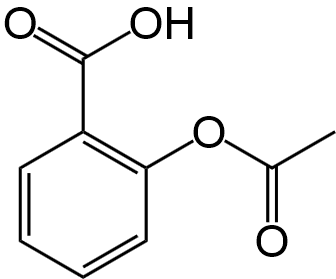
\includegraphics[height=10em]{Aspirin-skeletal.png}
		\caption{아스피린의 분자와 구조식}
		\label{fig:asp_ske}
	\end{figure}
	
	\paragraph{합성법}
	아스피린의 합성 방법에는 다양한 방법이 있다.
	버드나무 껍질에서 추출해낸 살리실산을 산 촉매를 이용하여
	아세트산과 에스터화 반응을 일으켜 합성하는 방법이 있다.
	\begin{figure}[H]
		\centering
		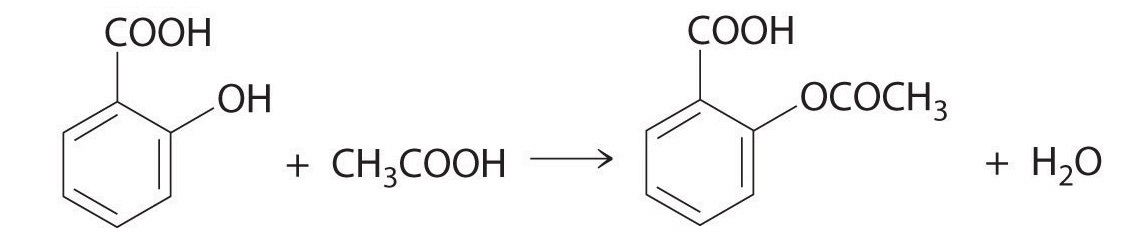
\includegraphics[width=\textwidth]{averillfwk-eq14_005_2.jpg}
		\caption{살리실산과 아세트산을 이용한 아세틸살리실산 합성 구조식}
		\label{fig:asp_form1}
	\end{figure}
	
	이 방법의 단점은, 아세트산과 생성된 물에 의해 산성 용액이 만들어지므로
	만들어진 아세틸살리실산이 다시 분해되는 일이 일어나
	수득률이 감소하게 된다는 점이다.
	
	독일의 제약회사 바이엘에서 아세틸살리실산의 수득률을 높이기 위해
	사용한 방법은 아세트산 대신 아세트산 무수물을 사용하고,
	산 촉매를 이용하는 방법이다.
	\begin{figure}[H]
		\centering
		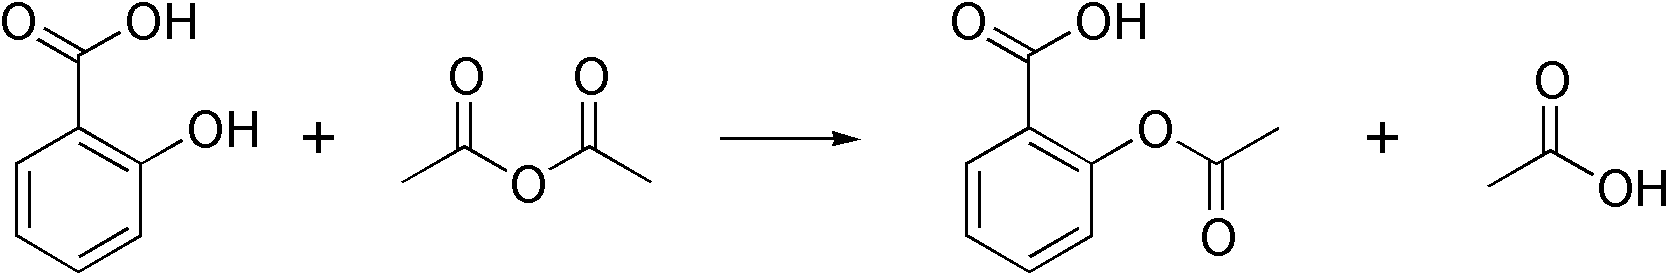
\includegraphics[width=\textwidth]{Aspirin_synthesis.png}
		\caption{살리실산과 아세트산 무수물을 이용한 아스피린 합성법}
		\label{fig:asp_form2}
	\end{figure}
	
	아세트산 무수물을 이용한 아스피린 합성 방법에는 산 촉매를 이용한다.
	\ce{H^{+}}가 무수아세트산에 결합하여 반응이 더 쉽게 이루어지도록 한다.
	결합한 양성자는 살리실산과 아세트산 무수물이 결합한 물질에서
	아세트산이 빠져나오면서 같이 빠져나온다.
	자세한 과정은 그림 \ref{fig:asp_form3}\과 같다.
	\begin{figure}[H]
		\centering
		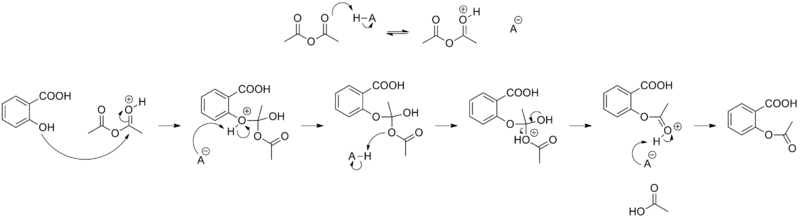
\includegraphics[width=\textwidth]{800px-Acetylation_of_salicylic_acid,_mechanism.png}
		\caption{산 촉매를 사용하는 살리실산, 아세트산 무수물의 아스피린 합성법}
		\label{fig:asp_form3}
	\end{figure}
	
	이번 실험에서는 \SI{85}{\percent} 인산을 산 촉매로 이용한다.
	
	\paragraph{약리 작용}
	아스피린은 항염증제와 항응고제로 작용한다.
	이 원리는, 아세틸살리실산이 살리실산으로 흡수될 때
	대뇌피질로 통증을 전달하는 데에 관여하는 물질인
	COX 효소의 생성을 저해한다.
	항염증제의 역할은 다른 항염증제와 메커니즘이 똑같다.
	항응고제 역할의 경우에는 COX 효소는 두 종류가 있는데
	하나가 혈액응고에 관여하는 COX-1이기 때문에 생기는 것이다.
	
	\paragraph{부작용}
	이러한 항응고 성질 때문에 부작용이 생기기도 한다.
	출혈을 동반한 환자들이나 혈우병이 있는 환자 등에게는
	아스피린을 처방하는 것이 오히려 역효과를 낼 수 있다.
	게다가 일반 사람에게도 이 응고를 막는 작용은
	위궤양을 유발할 수 있기 때문에 부작용이 많은 편이다.
	또한, 알레르기 천식 또한 종종 유발하며,
	만 14세 미만의 어린이가 복용하면 심각한 뇌손상을 일으키는
	라이 증후군이 발생할 가능성이 있으므로 반드시 어른만 복용해야 한다.
	
	\subsubsection{에스터화 반응}
	카복실산 혹은 카복실 무수물이 알코올과 반응하여
	에스터가 생성되는 반응으로, 산성 용액에서 매우 빠르게 일어난다.
	
	살리실산은 하이드록시기(\ce{-OH})를 가지고 있으므로
	살리실산을 카복실산인 아세트산 또는 아세트산 무수물과
	에스터화 반응을 일으켜 아스피린을 합성할 수 있다.
	
	\paragraph{에스터}
	유기산 또는 무기산과 알코올에서
	물을 잃고 생기는 구조를 가진 화합물을 일반적으로 에스터라고 한다.
	보통 에스터라고 하면 카복실산에스터를 가리키는데,
	이는 \ce{R-COO-R^{$\prime$}}의 구조를 갖는다.
	
	아스피린은 벤젠기에 \ce{COO-CH_{3}}가 붙은 카복실산에스터이다.
	
	\subsubsection{염화철(III) 정색 반응}
	페놀류 검출에 이용되는 반응이다. 페놀을 포함하고 있는 물질에
	염화철(III)(\ce{FeCl_{3}}) 수용액을 떨어뜨리면
	색이 보라색 또는 붉은색으로 변한다.
	이는 \ce{Fe^{3+}} 이온이 페놀의 \ce{O}와 결합하여
	특정한 색을 나타내기 때문이다.
	\begin{figure}[H]
		\centering
		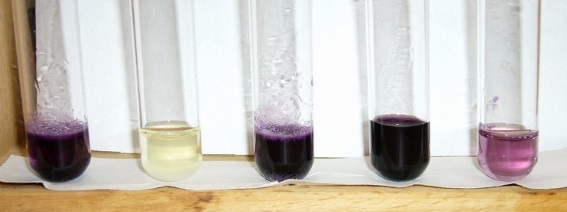
\includegraphics[scale=1]{noname02.jpg}
		\caption{여러 가지 화합물의 염화철 정색 반응 결과}
		\label{fig:fe3}
	\end{figure}
	
	염화철과 반응한 물질은 보라색을 띠고,
	반응하지 않은 물질은 보라색을 띠지 않는다.
	그림 \ref{fig:fe3}의 맨 오른쪽은 두 물질의 혼합물로, 옅은 보라색을 띤다.
	
	살리실산의 경우 페놀을 포함하고 있으므로
	염화철 정색 반응을 일으키면 색이 보라색으로 변한다.
	하지만 아스피린은 페놀을 형성하는 \ce{-OH}가 에스터화되어
	페놀이 없으므로 색이 변하지 않는다.
	
	\subsection{유의 사항}
	\begin{itemize}
		\item 실험이 끝난 후 폐수는 유기물 폐수통에 회수하고,
		유리 및 도자기류 기구(특히 정제한 침전을 거른 뷰흐너 깔때기)는
		즉시 절차대로 깨끗이 씻어둔다.
		\item 이 실험에서 합성한 아스피린은 절대 복용하지 않는다.
		\item 다음 실험을 위해 정제를 마친 아스피린은 버리지 말고 반드시 밀폐 용기에 보관해둔다.
	\end{itemize}
	
	\section{기구 및 시약}
	
	\subsection{실험 기구}
	\SI{50}{\milli\litre} 삼각 플라스크(Erlenmeyer flask),
	\SI{5}{\milli\litre} 눈금 피펫(measuring pipet),
	\SI{20}{\milli\litre} 눈금 실린더(graduated cylinder),
	디지털 물중탕(water bath; 가열판 기능 포함), 목장갑(cotton gloves),
	얼음 중탕(ice bath), 세척병(washing bottle), 오븐(drying oven),
	뷰흐너 깔때기(Büchner funnel), 거름종이(filter paper),
	감압 플라스크(suction flask), 감압기(aspirator), 흄 후드(fume hood)
	
	\subsection{실험 시약}
	살리실산(salicylic acid), 아세트산 무수물(acetic anhydride),
	\SI{85}{\percent} 인산(phosphoric acid), 증류수,
	에틸 에터(ethyl ether), 석유 에터(petroleum ether)
	
	\subsubsection{에틸 에터, 석유 에터}
	에틸 에터와 석유 에터는 매우 예민한 인화성 물질이므로, 가열판 주위에서 취급하지 않도록 한다.
	
	\subsubsection{아세트산 무수물}
	아세트산 무수물은 식초 냄새가 난다. 또한, 과량의 아세트산 무수물에 물을 가하여 분해하면, 뜨거운 아세트산 증기가 발생하므로 유의한다.
	
	\section{실험 과정}
	
	\subsection{아스피린의 합성}
	\begin{enumerate}
		\item 살리실산 \SI{2.5}{\gram}을 \SI{0.001}{\gram}까지 정확히 
		달아 \SI{50}{\milli\litre} 삼각 플라스크에 넣는다.
		\item 아세트산 무수물 \SI{3.0}{\milli\litre}를
		플라스크 벽에 묻은 살리실산을 모두 씻어낼 수 있도록
		벽을 따라 흘러내리는 방법으로 가한다.
		\item 플라스크에 \SI{85}{\percent} 인산 
		\unitrange{3}{4}{방울}을 첨가한 뒤 흄 후드 안에 설치한 
		\SIrange{70}{85}{\degreeCelsius} 물중탕에 고정시킨 채 
		\unit{15}{분} 간 반응시킨다.
		\item 증류수 \SI{2}{\milli\litre}를 조심스럽게 가하여
		반응하지 않고 남아있는 아세트산 무수물을 분해시킨다.
		\item 더 이상 아세트산 증기가 발생하지 않으면
		삼각 플라스크를 목장갑을 착용하고 물중탕에서 꺼내어
		증류수 \SI{20}{\milli\litre}를 가한 후
		실온까지 냉각시킨다(만일 이 과정으로 아스피린 결정이
		저절로 생기지 않으면 유리 막대로 플라스크 안쪽 벽을 긁어주면서
		얼음 중탕으로 냉각시킨다. 단, 결정이 충분히 생긴다면
		얼음 중탕을 쓰지 않는 것이 좋다).
		시간 절약을 위해 삼각 플라스크를 냉각하는 동안
		가열판의 온도를 조절하여 물중탕의 온도를
		\SI{50}{\degreeCelsius}로 재설정한다.
		\item 생성된 결정을 감압 여과로 걸러낸 뒤 \SI{5}{\milli\litre}의
		차가운 증류수로 씻고, 질량을 측정해둔 다른 거름종이로 옮겨
		\SI{70}{\degreeCelsius} 오븐에서 10분간 건조시켜 수득률을 계산한다.
	\end{enumerate}
	
	\subsection{아스피린의 정제}
	\begin{enumerate}
		\item 합성한 아스피린 \SI{1.0}{\gram} 정도를 덜어서
		\SI{50}{\milli\litre} 삼각 플라스크에 넣고
		에틸 에터 \SI{15}{\milli\litre}를 가한 뒤
		\SI{50}{\degreeCelsius} 물중탕으로 가열하여 녹인다.
		만일 녹지 않는 물질이 있으면 \SI{5}{\milli\litre} 정도의
		에틸 에터를 더 가해 완전히 녹인다(이 때 플라스크를 흔들거나
		유리막대로 젓지 않는다).
		\item 아스피린이 다 녹으면 석유 에터 \SI{15}{\milli\litre}를 
		가한 뒤 얼음 중탕에 담가 두어 침전이 생기도록 한다.
		역시 플라스크를 흔들거나 저으면 안 된다.
		\item 생성된 침전을 거르고 소량의 차가운 석유 에터로 씻은 뒤
		다른 거름종이에 옮겨 말린다.
	\end{enumerate}
	
	\subsection{합성 및 정제한 아스피린의 녹는점 비교}
	\begin{enumerate}
		\item DSC sample pan 두 개를 준비하여 정제 전후의 아스피린을
		각각 \SI{3.0}{\milli\gram} 정도씩 평평하게 집어넣고
		뚜껑을 덮은 뒤 프레스로 눌러 녹는점 측정 준비를 한다.
		\item DSC로 각각의 녹는점을 측정한다.
		\item 측정된 그래프와 미리 측정해둔 시약용 아세틸살리실산의 그래프를
		USB에 저장해 와서 상호 비교한다.
	\end{enumerate}
	
	\section{실험 결과}
	
	\subsection{아스피린의 합성}
	실험을 통해 측정한 실험에 사용한 살리실산의 질량과 빈 거름종이의 질량,
	아스피린을 옮기고 건조한 뒤 측정한 질량은 다음과 같다.
	\begin{itemize}
		\item 살리실산 질량 : \SI{2.550}{\gram}
		\item 빈 거름종이 질량 : \SI{0.680}{\gram}
		\item 건조 거름종이 질량 : \SI{4.116}{\gram}
	\end{itemize}
	
	살리실산과 아스피린의 분자량은 다음과 같다.
	\begin{itemize}
		\item 살리실산의 분자량 : 138
		\item 아스피린의 분자량 : 180
	\end{itemize}
	
	사용한 아세트산 무수물의 몰수가 살리실산보다 커
	살리실산이 전부 반응하여 아스피린이 되므로, 이론적 산출량은
	식 \ref{eq:eq1}로 구할 수 있다.
	\begin{gather}
		(\text{이론적 산출량}) = (\text{살리실산의 질량})
		\div (\text{살리실산의 분자량}) \times (\text{아스피린의 분자량})
		\label{eq:eq1}
	\end{gather}
	
	측정값을 통해 계산한 이론적 산출량과 실 산출량, 그리고 이를 이용해 계산한
	수득률은 다음과 같다.
	\begin{itemize}
		\item 이론적 산출량 : \SI{3.326}{\gram}
		\item 실 산출량 : \SI{3.436}{\gram}
		\item 수득률 : \SI{103.3}{\percent}
	\end{itemize}
	
	합성 후 염화철(III)을 이용하여 합성한 아스피린에 정색 반응을 일으킨 결과는
	다음과 같다.
	\begin{figure}[H]
		\centering
		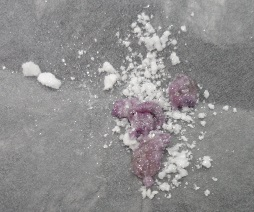
\includegraphics[scale=1]{noname03.jpg}
		\caption{합성한 아스피린에 염화철 정색 반응을 진행한 결과}
		\label{fig:fe3_2}
	\end{figure}
	
	정색 반응 결과 색이 옅은 보라색으로 변했다.
	
	\subsubsection{합성 및 정제한 아스피린의 녹는점 비교}
	합성, 정제한 아스피린의 DSC 측정은 진행하지 못하였다.
	
	\section{관찰 및 토의}
	
	\subsection{아스피린의 수득률}
	이번 실험에서는 수득률이 \SI{100}{\percent}가 넘었다.
	수득률 증가, 감소 원인을 생각해보고, 어느 요인이 영향을 미쳤을지 분석한다.
	
	\subsubsection{수득률 증가 요인}
	
	\paragraph{여과 후 건조}
	여과를 진행한 아스피린을 건조한 후 무게를 잴 때, 미처 건조가 되지 않아
	거름종이와 아스피린에 물이 남아 있었다면 무게가 증가했을 것이다.
	
	실제로 이번 실험에서는 시간이 부족하여 충분한 건조 시간을 갖지 못했다.
	따라서 이 요인은 수득률에 영향을 미쳤을 것이다.
	
	\paragraph{불순물}
	실험 과정에서 불순물이 첨가되거나 하면, 정제 과정을 거치지 않았기 때문에 무게가 증가한다. 그러나 이번 실험에서는 불순물의 양이 수득률에 큰 영향을 미치지는 않았을 것으로 생각된다.
	
	\subsubsection{수득률 감소 요인}
	
	\paragraph{반응의 미완결}
	살리실산과 아세트산 무수물이 반응하여 아세틸살리실산을 만드는 반응이
	완결되지 않고 일부 살리실산이 그대로 남아있었다면,
	반응하여 아세틸기를 첨가해주어야 할 아세틸살리실산이 가수 분해되어
	없어지므로 무게가 감소하였을 것이다
	
	이번 실험에서 합성한 아스피린에 염화철 정색반응을 진행했을 때
	옅은 보라색이 나왔던 것으로 보아, 반응이 완결되지 않았음을 알 수 있다.
	이는 수득률을 감소시킬 뿐 아니라, 순도를 낮게 하므로
	순 수득률은 더 낮아지는 결과를 얻게 된다.
	
	\paragraph{실험 진행 중의 유실}
	실험 과정에 물질들을 옮겨 담는 과정이 많았다.
	이 과정에서 흘리거나 하여 일부가 유실되었다면,
	수득률이 감소하였을 것이다. 이번 실험에서도 시약을 옮겨 담는 과정에서
	약간의 시약의 손실이 있었다.
	
	\subsection{아세트산 무수물을 대체할 수 있는 물질}
	아세트산 무수물 대신 아실 할라이드를 사용하여
	반응을 진행할 수 있다.
	
	살리실산과 아실 할라이드를 반응시키면,
	아실 할라이드가 살리실산에 아실기를 제공하여 아스피린이 합성된다.
	\begin{figure}[H]
		\centering
		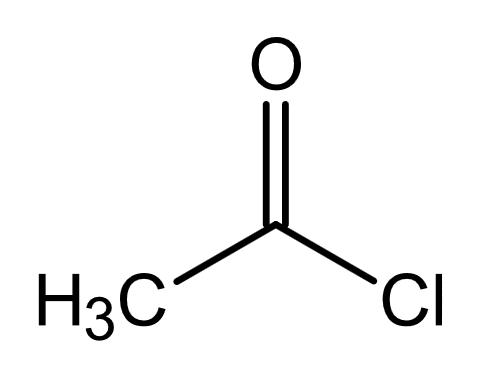
\includegraphics[height=10em]{Acetyl_chloride.png}
		\caption{아실 할라이드의 구조식}
		\label{fig:acyl_hal}
	\end{figure}
	
	\subsection{아스피린의 정제}
	이 실험에서는 아스피린을 에틸 에터와 석유 에터에 녹여
	재결정을 하는 방법으로 아스피린을 정제하였다.
	여기서 아스피린의 구조식을 다시 한 번 보자.
	\begin{figure}[H]
		\centering
		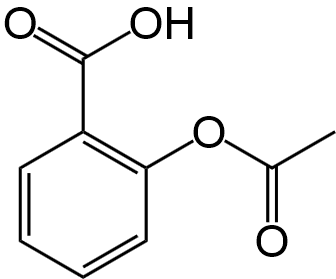
\includegraphics[height=10em]{Aspirin-skeletal.png}
		\caption{아스피린의 구조식}
	\end{figure}
	
	아스피린은 벤젠 고리를 포함하고 있다. 따라서 유기 용매에 잘 녹으므로, 유기 용매인 에터를 이용하여 재결정을 진행하였다.
	
	\section{결론 및 제언}
	\begin{itemize}
		\item 물질의 합성 과정에 있어서 중요한 것 중 하나는
		반응의 완결 조건이다. 조건에는 반응물의 양이 과량인지,
		농도가 적당한지뿐 아니라 반응 시간도 있다.
		이번 실험에서도 충분한 시간 동안 실험을 진행하지 못해
		아스피린 합성 반응이 완결되지 못하고,
		여과한 아스피린을 전부 말리지 못하여 실험 오차가 발생하고
		실 수득률이 낮아지는 결과를 얻었다.
		연구를 진행할 때나, 실제 제조 공정을 만들 때에는
		먼저 시간에 따른 반응이 진행되는 정도를 먼저 실험하여
		적절한 반응 시간을 찾아야 한다.
	\end{itemize}
	
	%\begin{thebibliography}{00}
	%\end{thebibliography}
			
\end{document}